% Copyright 2009--2010  Ed Bueler

\section{heat analogy \& numerics}

\subsection{analogy}

\begin{frame}{compare to heat equation}
\label{slide:heatcompare}

\small
\begin{columns}
\begin{column}{0.6\textwidth}
\begin{itemize}
\item recall Newton's law of cooling
	$$\frac{dT}{dt} = -\mu (T-T_{\text{ambient}})$$
where $T$ is temperature and $\mu$ relates to material and geometry of object
\item Newton's law for segments of an insulated rod:
\begin{align*}
\frac{dT_j}{dt} &= -\tilde \mu \left(T_j - \frac{1}{2} (T_{j-1} + T_{j+1}) \right) \\
	&= \frac{\tilde \mu}{2} \left(T_{j-1} - 2 T_j + T_{j+1}\right) 
\end{align*}
(where $\tilde \mu$ is material constant proportional to $\Delta x^{-2}$)
\item this suggests finite difference approximation of a PDE:
	$$T_t = D T_{xx}$$
\end{itemize}
\end{column}
\begin{column}{0.4\textwidth}
\hfill
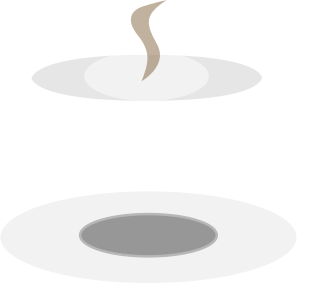
\includegraphics[width=0.5\textwidth]{pdffigs/coffee}
\vspace{0.7in}
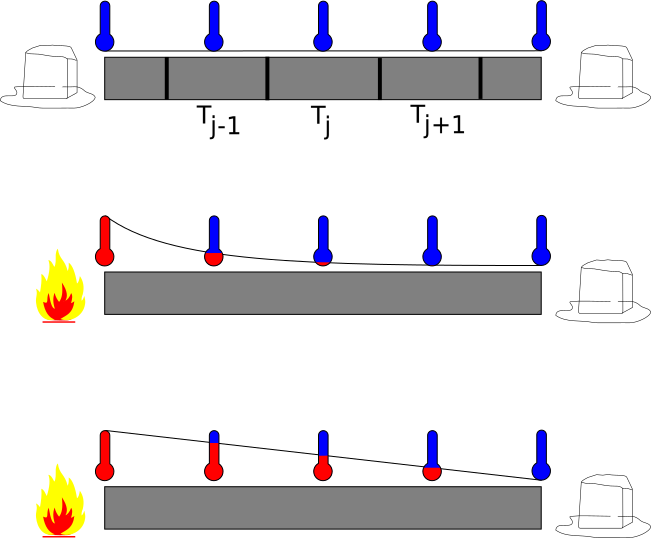
\includegraphics[width=1.0\textwidth]{pdffigs/heatconduction}

%COFFEE: \hfill \tiny (\emph{user:Assassingr, wiki commons image})
%HEAT:  \hfill \tiny (\emph{Christophe Dang Ngoc Chan, wiki commons image})
\end{column}
\end{columns}
\end{frame}


\begin{frame}{compare to heat equation 2}

\small
continuum version:
\begin{columns}
\begin{column}{0.6\textwidth}
\begin{itemize}
\item Fourier rewrote Newton's law as heat flux in continua: $\mathbf{q} = - k \grad u$
\item by conservation of energy, allowing an additional source of heat $f$, get heat equation:
	$$\rho c u_t = f + \Div (k \grad u)$$
\end{itemize}
\end{column}
\begin{column}{0.4\textwidth}
\animategraphics[autoplay,loop,height=2.5cm]{4}{anim/heatmelt}{0}{16}
\end{column}
\end{columns}


\begin{itemize}
\item set $D=k/(\rho c)$ and $M=f/(\rho c)$:
\begin{empheq}[box=\fbox]{equation}
u_t = M + \Div (D\, \grad u) \label{heat}
\end{empheq}
\item this heat equation is a diffusive, time-dependent PDE, \emph{like the SIA model for ice sheets}
\end{itemize}
\end{frame}


\begin{frame}{analogy: SIA versus heat equation}

\begin{itemize}
\item side-by-side comparison:
\begin{center}
\begin{tabular}{cc}
\scriptsize SIA: $H(t,x,y)$ is ice thickness & \scriptsize heat: $u(t,x,y)$ is temperature \normalsize \\
	\boxed{H_t = M + \Div \left({\color{red}\Gamma H^{n+2} |\grad h|^{n-1}}\, \grad h \right)}  &  \boxed{u_t = M + \Div (D\, \grad u)}
\end{tabular}
\end{center}

\medskip
\item we identify the diffusivity in the SIA:
	$$D = {\color{red}\Gamma H^{n+2} |\grad h|^{n-1}}$$
\item non-sliding shallow ice flow \emph{diffuses} the ice because the flow is down the surface gradient

\bigskip
\item some issues with this analogy:
  \begin{itemize}
  \item[$\circ$]  $\grad H\ne \grad h$ when bed is not flat \dots so what?
  \item[$\circ$]  $D$ depends on solution $H(t,x,y)$ \dots how does that complicate the numerical solution method?
  \item[$\circ$]  $D\to 0$ at margin ($H\to 0$) and at dome ($|\grad h|\to 0$) \dots so what?
  \end{itemize}
\item I'll get back to these ``issues'', but now let's get our hands dirty and numerically solve the heat equation
\end{itemize}
\end{frame}


\subsection{finite differences}

\begin{frame}{finite differences for heat equation}

basic ideas of finite differences:
\begin{itemize}
\item for differentiable $f(x)$ and any $\Delta x$, \emph{Taylor} says
\small
	$$f(x+\Delta x) = f(x) + f'(x) \Delta x + \frac{1}{2} f''(x) \Delta x^2 + \frac{1}{3!} f'''(x) \Delta x^3 + \dots$$
\normalsize
\item you can replace ``$\Delta x$'' with other expressions, e.g.:
\small
\begin{align*}
f(x-\Delta x) &= f(x) - f'(x) \Delta x + \frac{1}{2} f''(x) \Delta x^2 - \frac{1}{3!} f'''(x) \Delta x^3 + \dots \\
f(x+2\Delta x) &= f(x) + 2 f'(x) \Delta x + 2 f''(x) \Delta x^2 + \frac{4}{3} f'''(x) \Delta x^3 + \dots
\end{align*}
\normalsize
\item basic finite difference idea for differential equations: \emph{combine expressions like these to approximate derivatives}
\item for all of these notes, grid points have equal spacing $\Delta x$
\end{itemize}
\end{frame}


\begin{frame}{finite differences for heat equation 2}

\begin{itemize}
\item \emph{partial} derivative expressions, for example with $u=u(t,x)$:
\small
\begin{align*}
u_t(t,x) &= \frac{u(t+\Delta t,x) - u(t,x)}{\Delta t} + O(\Delta t), \\
u_t(t,x) &= \frac{u(t+\Delta t,x) - u(t-\Delta t,x)}{2\Delta t} + O(\Delta t^2), \\
u_x(t,x) &= \frac{u(t,x+\Delta x) - u(t,x)}{\Delta x} + O(\Delta x), \\
u_x(t,x) &= \frac{u(t,x+\Delta x) - u(t,x-\Delta x)}{2\Delta x} + O(\Delta x^2), \\
u_{xx}(t,x) &= \frac{u(t,x+\Delta x) - 2 u(t,x) + u(t,x-\Delta x)}{\Delta x^2} + O(\Delta x^2)
\end{align*}
\normalsize
\item sometimes we want a derivative in-between grid points:
\small
	$$u_x(t,x+(\Delta x/2)) = \frac{u(t,x+\Delta x) - u(t,x)}{\Delta x} + O(\Delta x^2)$$
\normalsize
\item ``$+O(\Delta x^2)$'' is better than ``$+O(\Delta x)$'' if $\Delta x$ is a small number
\end{itemize}
\end{frame}


\begin{frame}{explicit scheme for heat equation}
\label{slide:explicit}

\begin{itemize}
\item recall 1D heat equation $u_t = D u_{xx}$
\item the \emph{explicit} scheme using notation $u_j^n \approx u(t_n,x_j)$, so
	$$\frac{u_j^{n+1} - u_j^n}{\Delta t} = D\,\frac{u_{j+1}^n - 2 u_j^n + u_{j-1}^n}{\Delta x^2}$$
\item let $\nu = D \Delta t / (\Delta x)^2$, so
	$$u_j^{n+1} = \nu u_{j+1}^n + (1 - 2 \nu) u_j^n + \nu u_{j-1}^n$$
\end{itemize}

\begin{columns}[b]
\begin{column}{0.70\textwidth}
\begin{itemize}
\item scheme has stencil at right \large $\to$ \normalsize
\item advantage over implicit (later): $u_j^{n+1}$ is determined by \emph{known} quantities at time $t_n$
\bigskip
\end{itemize}
\end{column}
\begin{column}{0.3\textwidth}
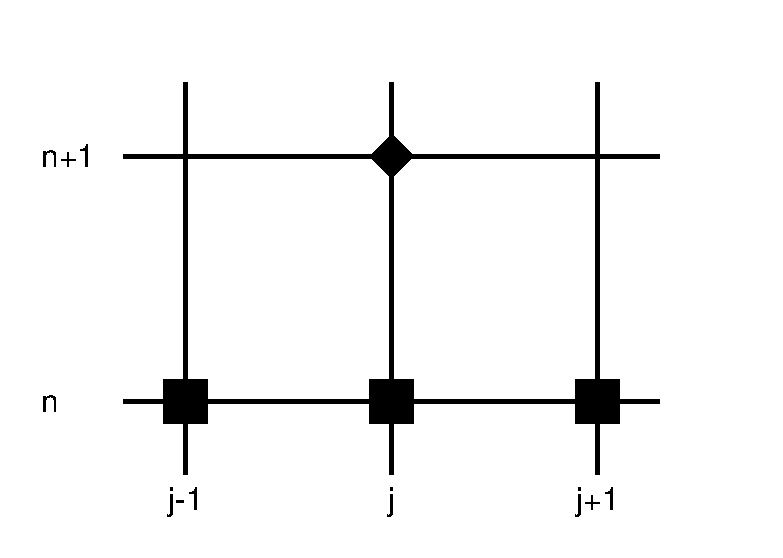
\includegraphics[width=1.0\textwidth]{pdffigs/expstencil}
\end{column}
\end{columns}
\end{frame}


\begin{frame}{explicit scheme for heat equation 2}

\begin{itemize}
\item in 2D we write $u_{jk}^n \approx u(t_n,x_j,y_k)$
\item the 2D explicit scheme for the $M=0$ heat equation $u_t = D(u_{xx} + u_{yy})$ is
\small
	$$\frac{u_{jk}^{n+1} - u_{jk}^n}{\Delta t} = D\,\left(\frac{u_{j+1,k}^n - 2 u_{jk}^n + u_{j-1,k}^n}{\Delta x^2} + \frac{u_{j,k+1}^n - 2 u_{jk}^n + u_{j,k-1}^n}{\Delta y^2}\right)$$
\normalsize
\item or, with $\nu^x := D \Delta t / (\Delta x)^2$ and $\nu^y := D \Delta t / (\Delta y)^2$,
\small
\begin{align*}
u_{jk}^{n+1} &= (1 - 2 \nu^x - 2 \nu^y) u_{jk}^n + \nu^x \left(u_{j+1,k}^n + u_{j-1,k}^n\right) + \nu^y \left(u_{j,k+1}^n + u_{j,k-1}^n\right)
\end{align*}
\end{itemize}

\begin{columns}[b]
\begin{column}{0.62\textwidth}
note: new value $u_{jk}^{n+1}$ is \emph{average} (is it?) of five quantities at old time $t_n$ \qquad $\longrightarrow$
\end{column}
\begin{column}{0.38\textwidth}
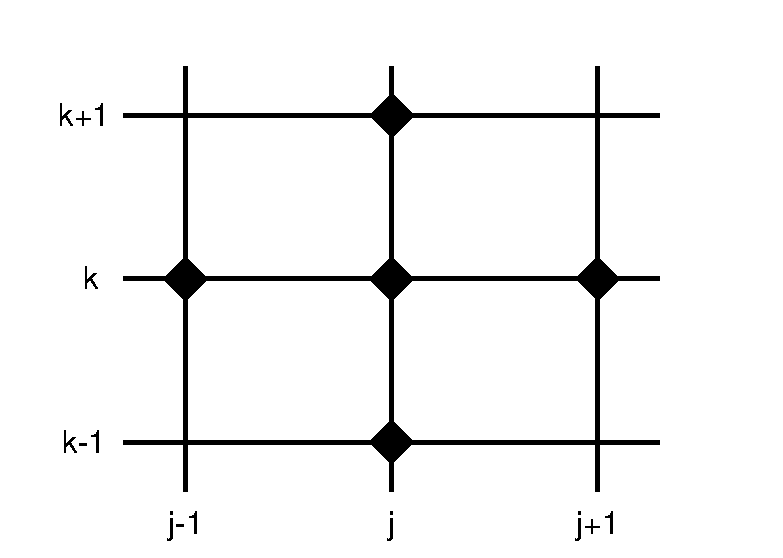
\includegraphics[width=1.1\textwidth]{pdffigs/exp2dstencil}
\end{column}
\end{columns}
\end{frame}


\begin{frame}{implementation}
\label{slide:heatmatlab}

\minput{heat}

\small
\begin{itemize}
\item solves $u_t = D(u_{xx} + u_{yy})$ on square $-1 < x < 1$, $-1 < y < 1$
\item choice: gaussian initial condition
\item ``colon notation'' removes loops over spatial variables
\item to approximate $u$ on $30\times 30$ spatial grid, with $D=1$ and $N=20$ steps of length $\Delta t = 0.001$,

\texttt{>>  heat(1.0,30,30,0.001,20)}
\end{itemize}
\end{frame}


\begin{frame}{the look of success}

\begin{itemize}
\item solving $u_t = D(u_{xx} + u_{yy})$ on $30\times 30$ grid
\end{itemize}

\bigskip\bigskip
\begin{columns}
\begin{column}{0.5\textwidth}
initial condition $u(0,x,y)$

\bigskip
\begin{center}
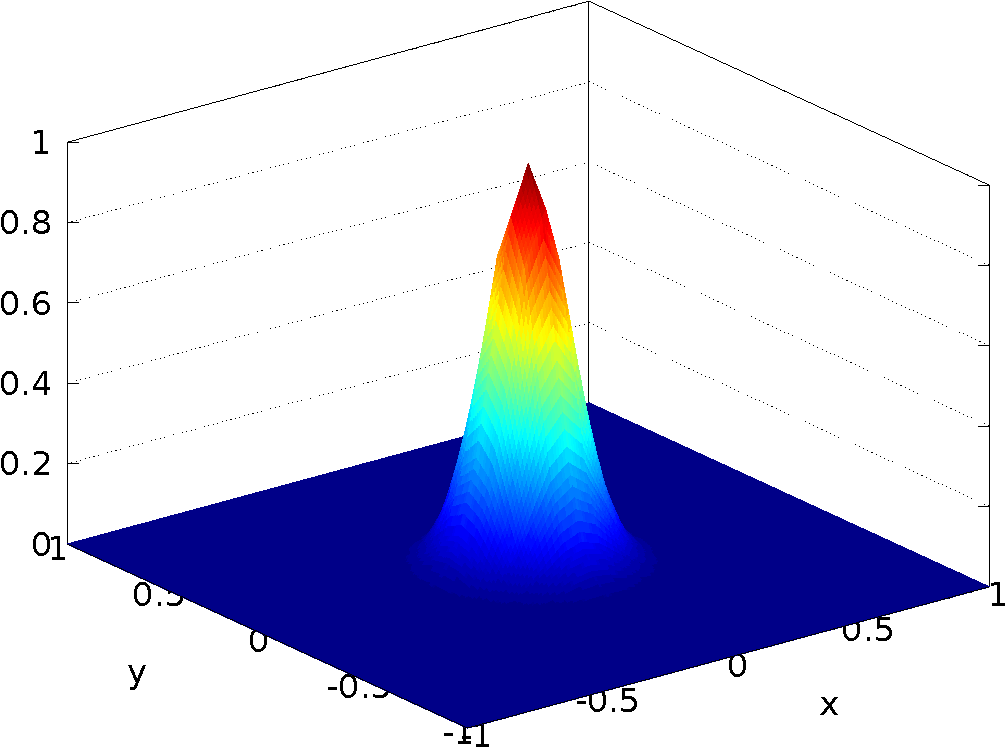
\includegraphics[width=1.0\textwidth]{photos/initialheat}
\end{center}
\end{column}
\begin{column}{0.5\textwidth}
approximate solution $u(t,x,y)$ at $t=0.02$ with $\Delta t=0.001$ 

\bigskip
\begin{center}
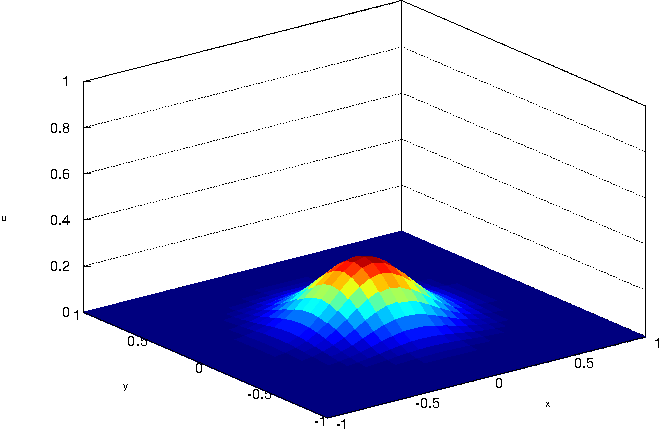
\includegraphics[width=1.0\textwidth]{photos/finalheat}
\end{center}
\end{column}
\end{columns}
\end{frame}


\begin{frame}{the look of instability}

\begin{itemize}
\item both figures are from solving $u_t = D(u_{xx} + u_{yy})$ on the same $50\times 50$ grid, at same final time and with same $D$, but with slightly different time steps
\end{itemize}

\bigskip
\begin{columns}
\begin{column}{0.5\textwidth}
\begin{center}
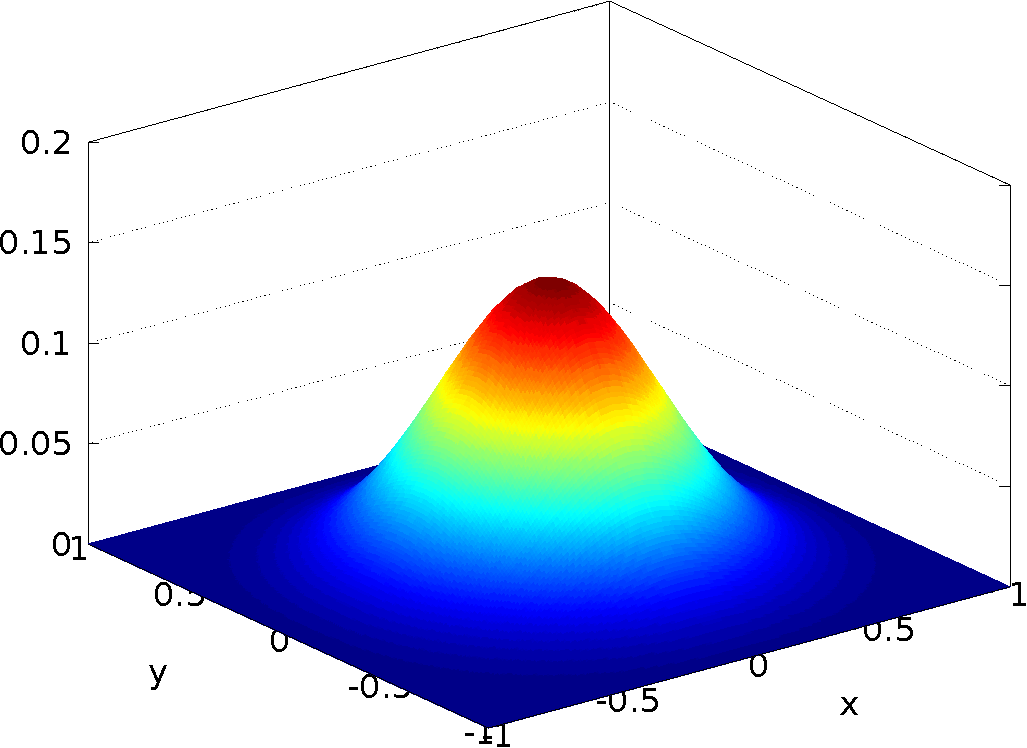
\includegraphics[width=1.0\textwidth]{photos/stability}
%$D=1,\Delta t = 0.00064286,\Delta x = \Delta y = 0.04$ so
  $$FIXME: see notes \frac{D\Delta t}{\Delta x^2}= 0.402$$
\end{center}
\end{column}
\begin{column}{0.5\textwidth}
\begin{center}
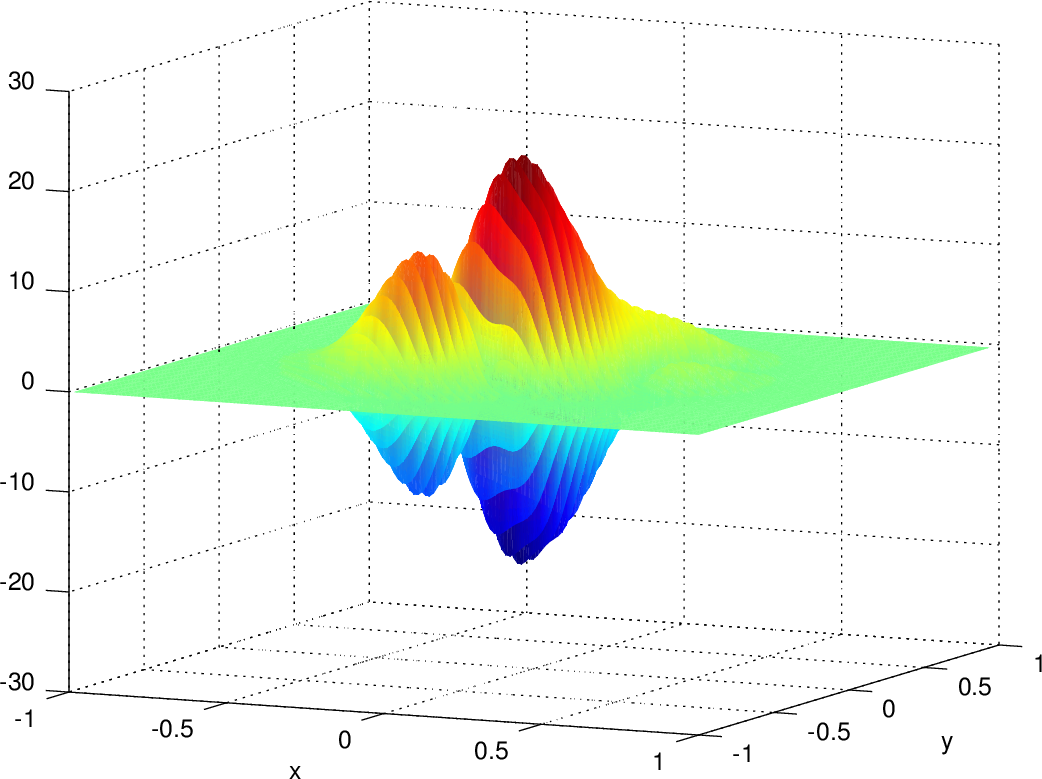
\includegraphics[width=1.0\textwidth]{photos/instability}
%$D=1,\Delta t = 0.001,\Delta x = \Delta y = 0.04$ so
  $$FIXME: see notes \frac{D\Delta t}{\Delta x^2}= 0.625$$
\end{center}
\end{column}
\end{columns}
\end{frame}


\begin{frame}{why unstable?}
\label{slide:maxprinc}

\begin{itemize}
\item the 1D first-order explicit scheme in the form 
	$$u_j^{n+1} = \nu u_{j+1}^n + (1 - 2 \nu) u_j^n + \nu u_{j-1}^n$$
gives new value $u_j^{n+1}$ as an \emph{average} of old values,
\item but it is only an average if the middle coefficient is positive:\footnote{recommended basic reference for finite differences, including stability: [Morton and Mayers, 2005]\nocite{MortonMayers}}
	$$1 - 2 \nu = 1 - 2 \frac{D\Delta t}{\Delta x^2} \ge 0$$
\item true averaging is always stable because averaged wiggles are smaller than the previous wiggles
\item ``positive coefficients'' is a \emph{sufficient} stability criterion
\item the same thing as a time-step restriction:
	$$\Delta t \le \frac{\Delta x^2}{2 D}$$
\end{itemize}
\end{frame}


\begin{frame}{\textsl{adaptive} implementation: guaranteed stability}

\minput{heatadapt}

\small
\begin{itemize}
\item same as \texttt{heat.m} except it gets the time step from:
	$$\frac{D\Delta t}{(\min\{\Delta x,\Delta y\})^2} \le \frac{1}{4}$$
\end{itemize}\end{frame}


\begin{frame}{alternative instability fix: implicitness}

\begin{columns}[T]
\begin{column}{0.7\textwidth}
\small
\begin{itemize}
\item explicit scheme is only ``conditionally stable'', but there are methods which are stable for \emph{any} positive time step $\Delta t$
\item the simplest such is \emph{first-order implicit} $\to$,
	$$\frac{u_j^{n+1} - u_j^n}{\Delta t} = D\,\frac{u_{j+1}^{n+1} - 2 u_j^{n+1} + u_{j-1}^{n+1}}{\Delta x^2}$$
\item another is \emph{Crank-Nicolson} $\to$; instead of $O(\Delta t,\Delta x^2)$ like first-order explicit and implicit, Crank-Nicolson is $O(\Delta t^2,\Delta x^2)$
\end{itemize}
\end{column}
\begin{column}{0.3\textwidth}
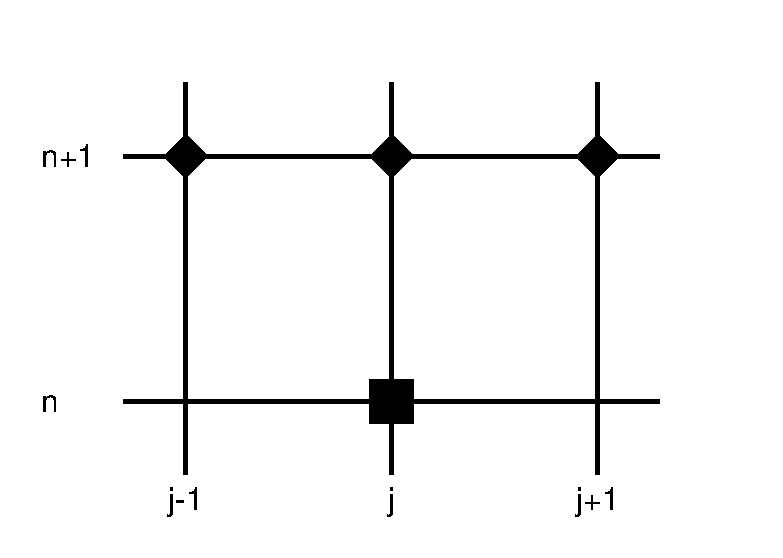
\includegraphics[width=1.2\textwidth]{pdffigs/impstencil}

\bigskip
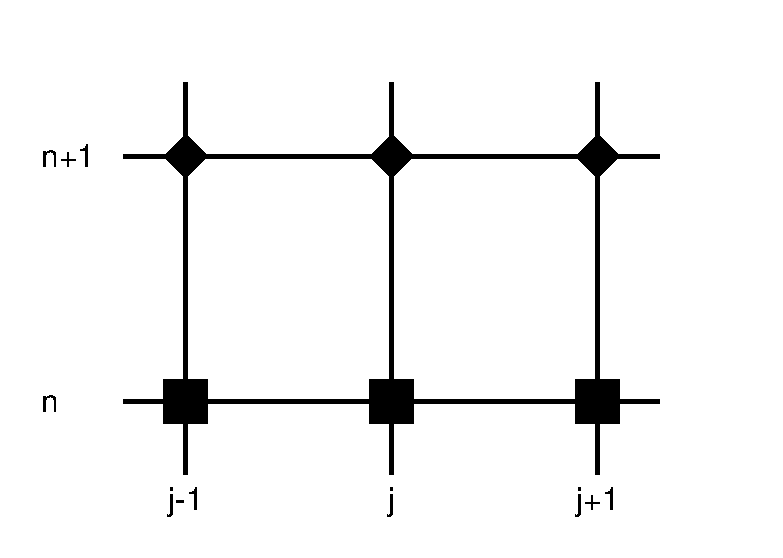
\includegraphics[width=1.2\textwidth]{pdffigs/cnstencil}
\end{column}
\end{columns}

\begin{itemize}
\small
\item \emph{but} for implicit and Crank-Nicolson methods you have to solve systems of equations to take each step
\medskip

\item \scriptsize Donald Knuth has advice for ice sheet modelers: \begin{quote}
\emph{We should forget about small efficiencies, say about 97\% of the time: premature optimization is the root of all evil}.
\end{quote}
\end{itemize}
\end{frame}


\begin{frame}{variable diffusivity and time steps}

\begin{itemize}
  \item recall analogy \qquad (SIA) $\leftrightarrow$ (heat eqn)
  \item the SIA has a diffusivity $D$ which varies in time and space, so by analogy:
  		$$u_t = M + \Div \left(D(t,x,y) \grad \right)$$
  \item the explicit method is conditionally stable with the ``same'' stability condition \emph{if} we evaluate diffusivity $D(t,x,y)$ at \alert{staggered} grid points:
  \scriptsize
\begin{align*}
\Div \left(D(t,x,y) \grad u\right) &\approx \frac{D_{j+1/2,k}(u_{j+1,k} - u_{j,k}) - D_{j-1/2,k}(u_{j,k} - u_{j-1,k})}{\Delta x^2} \\
	&\qquad + \frac{D_{j,k+1/2}(u_{j,k+1} - u_{j,k}) - D_{j,k-1/2}(u_{j,k} - u_{j,k-1})}{\Delta y^2}
\end{align*}
\end{itemize}

\vspace{-0.15in}
\small
\begin{columns}
\begin{column}{0.55\textwidth}
in stencil at right:
\begin{itemize}
\item[] diamonds: $u$
\item[] triangles: $D$
\end{itemize}
\end{column}
\begin{column}{0.45\textwidth}
\begin{center}
\vspace{-0.15in}
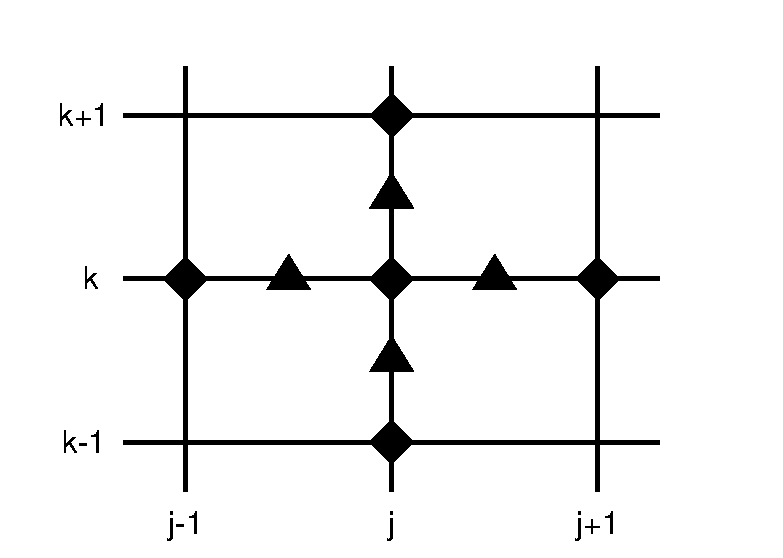
\includegraphics[width=1.0\textwidth]{pdffigs/diffstencil}
\end{center}
\end{column}
\end{columns}
\end{frame}


\begin{frame}
  \frametitle{general diffusion equation code}

\minput{diffusion}

\small
\begin{itemize}
\item solves abstract diffusion equation $u_t = \Div \left(D(x,y)\, \grad u\right)$
\item user must supply diffusivity on staggered grid
\end{itemize}
\end{frame}


\subsection{exact solutions}

\begin{frame}{on exact solutions}

\begin{itemize}
\item I am not quite done with the (heat) $\leftrightarrow$ (SIA) analogy
\item \dots I also want to use it to address exact solutions and verification

\bigskip
\item the two senses of ``solution'':
  \begin{itemize}
  \small
  \item[$\circ$] a \emph{solution} $u(t,x,y)$ of the heat equation is a function of time and space for which $u_t = M + \Div (D\, \grad u)$ is true
  \item[$\circ$] a \emph{solution} of the heat equation is a \emph{prediction} of that model
  \normalsize
  \end{itemize}
\item exact solutions are exact predictions of the model, but not exact predictions about nature
\item if we can only \emph{approximately} find solutions of a model then knowing a few exact solutions can help test and maintain the quality of the actual code that does the approximation \dots this is \emph{verification} [Wesseling, 2001]\nocite{Wesseling}
\end{itemize}
\end{frame}


\begin{frame}{exact solutions of heat equation}

\begin{itemize}
\item \emph{many} solutions to the heat equation are known, but one is ``fundamental'' to the time-dependent equation, namely the Green's function
\end{itemize}

\begin{columns}[b]
\begin{column}{0.5\textwidth}
\begin{itemize}
\small
\item as time goes it changes shape by shrinking the output (vertical) axis and simultaneously lengthening the input (horizontal) axis
\item \dots \emph{but otherwise it is the same shape}, so it is self-similar
\item there are solutions of the SIA just like this
\normalsize
\end{itemize}
\end{column}
\begin{column}{0.5\textwidth}
\begin{center}
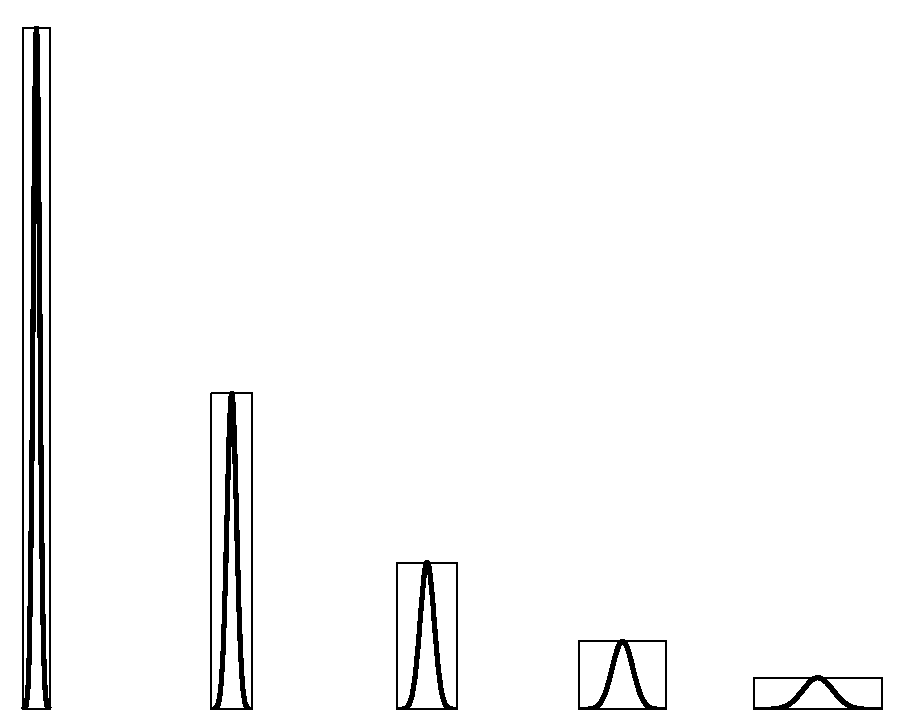
\includegraphics[width=1.0\textwidth]{pdffigs/heatscaling}

\emph{increasing time} \Large $\to$
\end{center}
\end{column}
\end{columns}
\end{frame}


\begin{frame}{finding the Green's function of the heat equation}

\begin{itemize}
\item the best-known way to find the Green's function of the heat equation is by Fourier transform, but we use a method which generalizes to the SIA
\item facts used to find it:
  \begin{itemize}
    \item[$\circ$] the Green's function starts at time $t=0$ with a \emph{delta function} at the origin $r=0$
    \item[$\circ$] the Green's function is angularly-symmetric:  $u$ is a function of the polar coordinate $r = \sqrt{x^2+y^2}$
    \item[$\circ$] calculus says: if $f=f(r)$ then $\grad^2 f = r^{-1} \left(r f'\right)'$
    \item[$\circ$] thus the heat equation in 2D, without additional heat sources, with constant diffusivity $D>0$, and for a function of $r$, is:
   $$u_t = D r^{-1} \left(r u_r\right)_r$$
  \end{itemize}
\item we use above facts to get Green's function by its ``similarity'' properties
\item \emph{but} we do not use the linearity of the heat equation
\end{itemize}
\end{frame}


\begin{frame}{finding a ``similarity'' solution of heat equation}
\label{slide:heatsim}

\small
\begin{itemize}
\item function $u(t,r)$ is replaced by function $\phi$ of one new variable $s$
\item input scaling: $s = t^{-\beta} r$
\item output scaling: $u = t^{-\alpha} \phi(s)$
\item chain rule says:
\begin{align*}
  u_t &= -\alpha t^{-\alpha-1} \phi - \beta t^{-\alpha-\beta-1} r \phi', \qquad u_r = t^{-\alpha-\beta} \phi', \qquad \text{etc.}
\end{align*}
\item so heat equation $u_t = D r^{-1} \left(r u_r\right)_r$ is replaced by:
	$$-\alpha \phi - \beta s \phi' = D s^{-1} t^{-2\beta+1} \left(\phi' + s \phi''\right)$$
\item choose $\boxed{\beta=1/2}$ so equation has no ``$t$'' and further simplify to
   $$-\frac{1}{2} \left[2 \alpha s \phi + s^2 \phi'\right] = D \left(s\, \phi'\right)'$$
\item choose $\boxed{\alpha = 1}$ so that quantity in square brackets simplifies to a derivative: $2 \alpha s \phi + s^2 \phi' = \left(s^2 \phi\right)'$
\end{itemize}
\end{frame}


\begin{frame}{finding a ``similarity'' solution of heat equation 2}

\small
\begin{itemize}
\item simplify and integrate, choose $C=0$, integrate again:
\begin{align*}
  - \frac{1}{2} s^2 \phi &= D\, s\,\phi' + C\\
  \phi' &= - \frac{s}{2D} \phi \\
  \phi(s) &= A e^{-s^2/(4D)}
\end{align*}
\item return to original variables, recalling $s = t^{-\beta} r$:
	$$u(t,r) = A\,t^{-1}\, e^{-r^2/(4Dt)} = A\,t^{-1}\, e^{-(x^2+y^2)/(4Dt)}$$
\item it is a spreading gaussian distribution
\item heat equation is linear so \emph{all} time-dependent solutions of the heat equation are convolutions with this solution \dots which is why it is \emph{fundamental}
\end{itemize}

\begin{center}
\animategraphics[autoplay,loop,height=2cm]{4}{anim/heatmelt}{0}{16}
\end{center}
\end{frame}


\begin{frame}{similarity solutions}

\begin{itemize}
\item \emph{conclusion from previous slides}: similarity variables for heat equation are
	$$s \stackrel{\text{\emph{input scaling}}}{\phantom{\Big|}=\phantom{\Big|}} t^{-\beta} x, \qquad u(t,x) \stackrel{\text{\emph{output scaling}}}{\phantom{\Big|}=\phantom{\Big|}} t^{-\alpha} \phi(s)$$
\item dimension dependence:
	\begin{tabular}{l|ccc}
	               & 1D & 2D & 3D \\ \hline
	input scaling ($t^{-\beta}$)   & $t^{-1/2}$ & $t^{-1/2}$ & $t^{-1/2}$ \\
	output scaling ($t^{-\alpha}$) & $t^{-1/2}$ & $t^{-1}$ & $t^{-3/2}$
	\end{tabular}
\end{itemize}
\begin{columns}
\begin{column}{0.6\textwidth}
\emph{historical note}:  In 1905 Einstein saw that the average distance traveled in time $t$ by particles in thermal motion goes like $\sqrt{t}$.  This is a microscopic explanation of the similarity variable $s = t^{-1/2}x$.
\end{column}
\begin{column}{0.4\textwidth}
\hfill 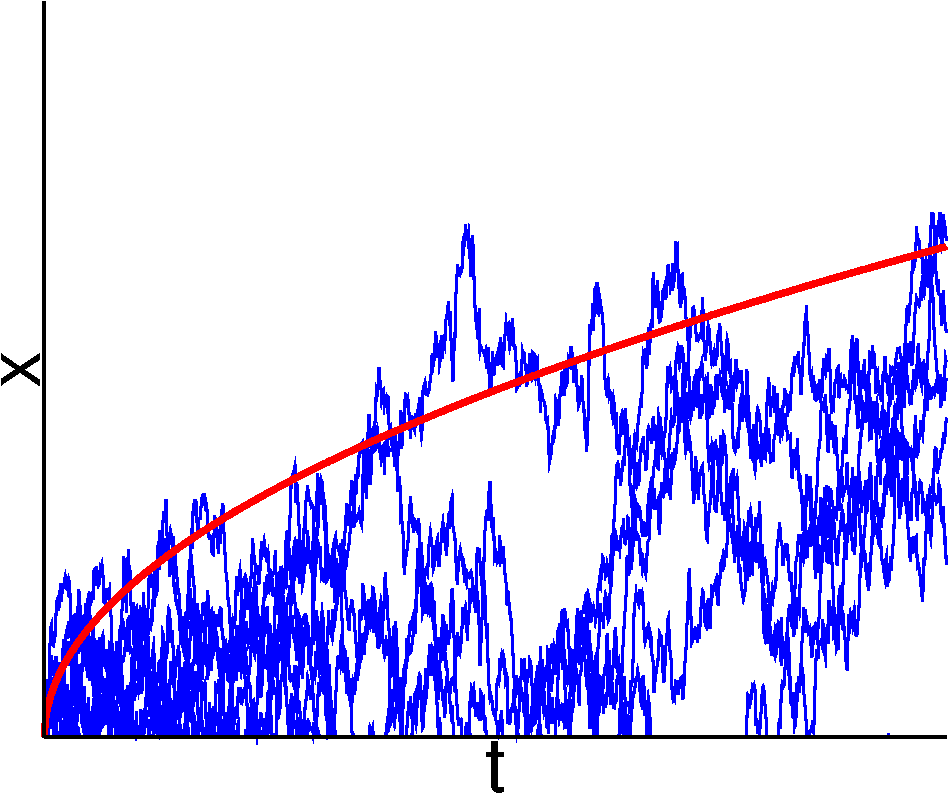
\includegraphics[width=0.8\textwidth]{photos/brownian}
\end{column}
\end{columns}
\end{frame}
